\documentclass[17pt,a4paper,landscape]{extarticle}
\usepackage[margin=2.35cm,top=0.12cm,left=1.05cm]{geometry}
\usepackage{amsmath}
\usepackage{amssymb}
\usepackage{tasks}
\usepackage{tikz}
\usepackage{xcolor}
\usepackage[sfdefault,lf]{FiraSans}
\renewcommand{\familydefault}{\sfdefault}
\setlength{\parindent}{0pt}
\pagestyle{empty}
\settasks{label=\textbf{\arabic*.}, label-width=2.2em, item-indent=2.95em, column-sep=2.1cm, after-item-skip=4.7em}
\renewcommand{\arraystretch}{1.15}
\everymath{\displaystyle}

\begin{document}
\sffamily
\boldmath

\boldmath

\boldmath

{\LARGE \textbf{Perimeter (shapes with straight edges only) --- Foundation}}
\begin{tasks}(3)
\task Find the perimeter.\\[0.4em]
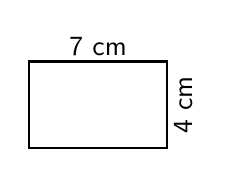
\begin{tikzpicture}[x=0.22cm,y=0.22cm,baseline=(current bounding box.center)]
  \draw[thick] (0,0) rectangle (8,5);
  \node at (4,5.9) {7 cm};
  \node[rotate=90] at (8.9,2.5) {4 cm};
\end{tikzpicture}
\task Find the perimeter.\\[0.4em]
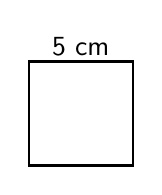
\begin{tikzpicture}[x=0.22cm,y=0.22cm,baseline=(current bounding box.center)]
  \draw[thick] (0,0) rectangle (6,6);
  \node at (3,6.9) {5 cm};
\end{tikzpicture}
\task Find the perimeter.\\[0.4em]
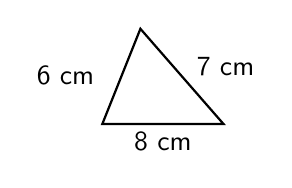
\begin{tikzpicture}[x=0.22cm,y=0.22cm,baseline=(current bounding box.center)]
  \coordinate (A) at (0,0);
  \coordinate (B) at (7,0);
  \coordinate (C) at (2.2,5.5);
  \draw[thick] (A)--(B)--(C)--cycle;
  \node at (3.5,-1.0) {8 cm};
  \node at (0.1,2.8) [left] {6 cm};
  \node at (4.9,3.3) [right] {7 cm};
\end{tikzpicture}
\task Find the perimeter.\\[0.4em]
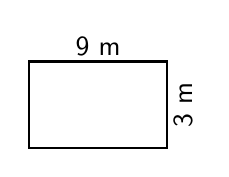
\begin{tikzpicture}[x=0.22cm,y=0.22cm,baseline=(current bounding box.center)]
  \draw[thick] (0,0) rectangle (8,5);
  \node at (4,5.9) {9 m};
  \node[rotate=90] at (8.9,2.5) {3 m};
\end{tikzpicture}
\task Find the perimeter.\\[0.4em]
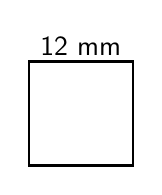
\begin{tikzpicture}[x=0.22cm,y=0.22cm,baseline=(current bounding box.center)]
  \draw[thick] (0,0) rectangle (6,6);
  \node at (3,6.9) {12 mm};
\end{tikzpicture}
\task Find the perimeter.\\[0.4em]
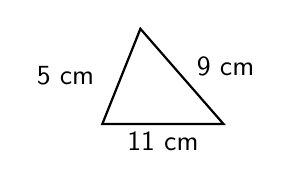
\begin{tikzpicture}[x=0.22cm,y=0.22cm,baseline=(current bounding box.center)]
  \coordinate (A) at (0,0);
  \coordinate (B) at (7,0);
  \coordinate (C) at (2.2,5.5);
  \draw[thick] (A)--(B)--(C)--cycle;
  \node at (3.5,-1.0) {11 cm};
  \node at (0.1,2.8) [left] {5 cm};
  \node at (4.9,3.3) [right] {9 cm};
\end{tikzpicture}
\task Find the perimeter.\\[0.4em]
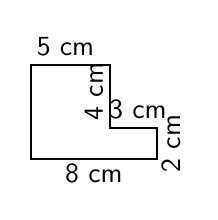
\begin{tikzpicture}[x=0.20cm,y=0.20cm,baseline=(current bounding box.center)]
  \draw[thick] (0,0)--(8,0)--(8,2)--(5,2)--(5,6)--(0,6)--cycle;
  \node at (4,-0.9) {8 cm};
  \node[rotate=90] at (8.9,1) {2 cm};
  \node at (6.8,3.2) {3 cm};
  \node[rotate=90] at (4.0,4.3) {4 cm};
  \node at (2.2,7.2) {5 cm};
\end{tikzpicture}
\task Find the perimeter.\\[0.4em]
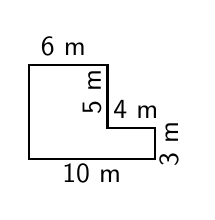
\begin{tikzpicture}[x=0.20cm,y=0.20cm,baseline=(current bounding box.center)]
  \draw[thick] (0,0)--(8,0)--(8,2)--(5,2)--(5,6)--(0,6)--cycle;
  \node at (4,-0.9) {10 m};
  \node[rotate=90] at (8.9,1) {3 m};
  \node at (6.8,3.2) {4 m};
  \node[rotate=90] at (4.0,4.3) {5 m};
  \node at (2.2,7.2) {6 m};
\end{tikzpicture}
\task Find the perimeter.\\[0.4em]
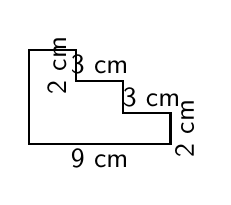
\begin{tikzpicture}[x=0.20cm,y=0.20cm,baseline=(current bounding box.center)]
  \draw[thick] (0,0)--(9,0)--(9,2)--(6,2)--(6,4)--(3,4)--(3,6)--(0,6)--cycle;
  \node at (4.5,-0.9) {9 cm};
  \node[rotate=90] at (9.9,1) {2 cm};
  \node at (7.8,3.0) {3 cm};
  \node at (4.5,5.1) {3 cm};
  \node[rotate=90] at (1.8,5.0) {2 cm};
\end{tikzpicture}
\task A rectangle is 14 cm long and 6 cm wide. Find its perimeter.
\task A square has side length 9 m. Find its perimeter.
\task A triangle has side lengths 12 cm, 12 cm and 7 cm. Find its perimeter.
\task The perimeter of a square is 28 cm. Find one side length.
\task The perimeter of a rectangle is 24 m. Its width is 5 m. Find its length.
\task A square has side length 15 cm. Find its perimeter.
\task A rectangle is 11 cm long and 4 cm wide. Find its perimeter.
\task A triangle has side lengths 6 m, 8 m and 9 m. Find its perimeter.
\task Explain how perimeter is different from area.
\end{tasks}

\end{document}
